\documentclass[11pt,a4paper]{article}
\usepackage[utf8]{inputenc}
\usepackage{amsmath,amssymb,amsthm}
\usepackage{graphicx}
\usepackage{geometry}
\geometry{margin=1in}
\usepackage{hyperref}
\usepackage{tikz}
\usetikzlibrary{arrows.meta,positioning,calc,fit,decorations.pathmorphing}
\usepackage{cite}

\usepackage[utf8]{inputenc}
\usepackage[T1]{fontenc}
\usepackage{amsmath,amssymb,bm}
\usepackage{tikz}
\usetikzlibrary{arrows.meta,calc,decorations.markings}
\usepackage{cite}
\documentclass[11pt]{article}
\usepackage[margin=1in]{geometry}
\usepackage{graphicx}
\usepackage{hyperref}
\usepackage{float}
\usetikzlibrary{arrows.meta, positioning}
\geometry{margin=2cm}

\begin{document}

\section*{TikZ Sketch: Dipole Fields}

\begin{center}
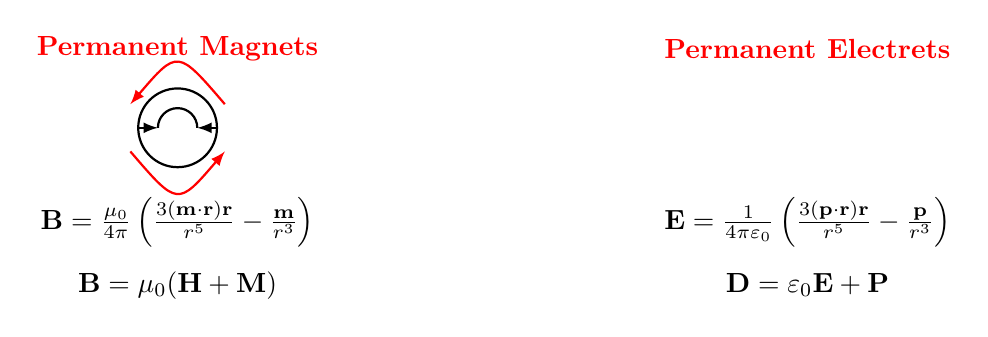
\begin{tikzpicture}[scale=1.0,>=latex]

% Headings
\node at (-4,5.5) {\textcolor{red}{\textbf{Permanent Magnets}}};
\node at (4,5.5) {\textcolor{red}{\textbf{Permanent Electrets}}};

% Magnetic dipole sketch
\draw[thick] (-4,4.5) circle (0.5);
\draw[thick] (-4.25,4.5) arc[start angle=180, end angle=0, radius=0.25];
\draw[->, thick] (-4.5,4.5) -- (-4.25,4.5);
\draw[->, thick] (-3.5,4.5) -- (-3.75,4.5);
\draw[->, thick, red] (-4.6,4.2) .. controls (-4,3.5) .. (-3.4,4.2);
\draw[->, thick, red] (-3.4,4.8) .. controls (-4,5.5) .. (-4.6,4.8);

% Magnetic field
\node at (-4,3.3) {$\mathbf{B} = \frac{\mu_0}{4\pi} \left( \frac{3(\mathbf{m} \cdot \mathbf{r})\mathbf{r}}{r^5} - \frac{\mathbf{m}}{r^3} \right)$};
\node at (-4,2.5) {$\mathbf{B} = \mu_0(\mathbf{H} + \mathbf{M})$};

% Electric field
\node at (4,3.3) {$\mathbf{E} = \frac{1}{4\pi\varepsilon_0} \left( \frac{3(\mathbf{p} \cdot \mathbf{r})\mathbf{r}}{r^5} - \frac{\mathbf{p}}{r^3} \right)$};
\node at (4,2.5) {$\mathbf{D} = \varepsilon_0 \mathbf{E} + \mathbf{P}$};

\end{tikzpicture}


\section*{TikZ Sketch: Fixed Swirl Flux, Shrinking Area $\Rightarrow$ Vortex Nucleation}

    \begin{center}
    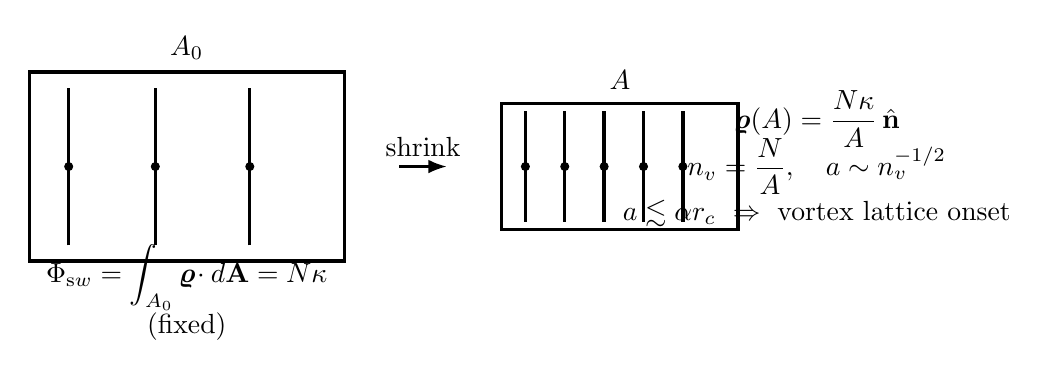
\begin{tikzpicture}[scale=1.0, >=Latex]
        % Left plate (area A0)
    \draw[very thick] (-5,1.2) rectangle (-1,-1.2);
    \node at (-3,1.5) {$A_0$};
    % Few vortices
    \foreach \x/\y in {-4.5/0.0, -3.4/0.6, -2.2/-0.4}{
        \draw[very thick] (\x,-1.0) -- (\x,1.0);
        \draw[fill=black] (\x,0) circle (0.05);
    }
    \node[align=center] at (-3,-1.6)
        {$\Phi_{\textrm sw}=\displaystyle\int_{A_0}\bm{\varrho}\!\cdot d\mathbf A = N\kappa$\\(fixed)};

    % Right plate (area A < A0)
    \draw[very thick] (1.0,0.8) rectangle (4.0,-0.8);
    \node at (2.5,1.1) {$A$};
    % Denser vortices
    \foreach \x/\y in {1.3/0.0, 1.8/0.4, 2.3/-0.3, 2.8/0.3, 3.3/-0.1}{
        \draw[very thick] (\x,-0.7) -- (\x,0.7);
        \draw[fill=black] (\x,0) circle (0.05);
    }
    % Arrow and labels
    \draw[->,thick] (-0.3,0) -- (0.3,0) node[midway,above] {shrink};
    \node[align=left] at (5.0,0.6)
        {$\bm{\varrho}(A)=\dfrac{N\kappa}{A}\,\hat{\mathbf n}$};
    \node[align=left] at (5.0,0.0)
        {$n_v=\dfrac{N}{A},\quad a\sim n_v^{-1/2}$};
    \node[align=left] at (5.0,-0.6)
        {$a\lesssim \alpha r_c\ \Rightarrow\ \text{vortex lattice onset}$};
    \end{tikzpicture}
    \end{center}
%===============================
% Figures (TikZ)
%===============================

\begin{figure}[t]
\centering
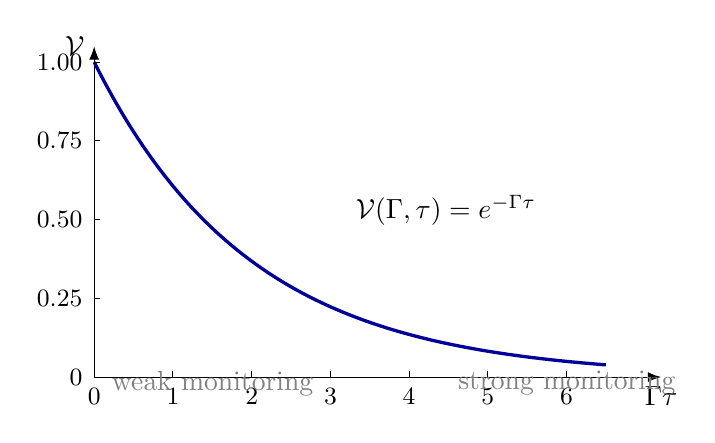
\begin{tikzpicture}[>=Latex,scale=1.0]
    % Axes
\draw[->] (0,0) -- (7.2,0) node[below] {$\Gamma\tau$};
\draw[->] (0,0) -- (0,4.2) node[left] {$\mathcal V$};
% Curve V = exp(-Gamma tau)
\draw[very thick,blue!60!black,domain=0:6.5,samples=200] plot(\x,{4*exp(-0.5*\x)});
% Ticks and labels
\foreach \x/\lab in {0/0,1/1,2/2,3/3,4/4,5/5,6/6}{
    \draw (\x,0) -- ++(0,0.08) node[below,yshift=-3pt] {\small \lab};
}
\foreach \y/\lab in {0/0,1/0.25,2/0.50,3/0.75,4/1.00}{
    \draw (0,\y) -- ++(0.08,0) node[left,xshift=-3pt] {\small \lab};
}
\node[above right] at (3.2,1.8) {$\mathcal V(\Gamma,\tau)=e^{-\Gamma\tau}$};
\node[below right,gray] at (0.1,0.2) {weak monitoring};
\node[below right,gray] at (4.5,0.2) {strong monitoring};
\end{tikzpicture}
\caption{Fringe visibility vs.\ which-way coupling in SST.
The parameter $\Gamma$ encodes EM impedance to the $\mathcal R$ phase (path information rate),
    $\tau$ is the transit time.
    Exponential decay of visibility reflects coherence loss prior to recombination.}
\label{fig:VvsGamma}
\end{figure}

\begin{figure}[t]
\centering
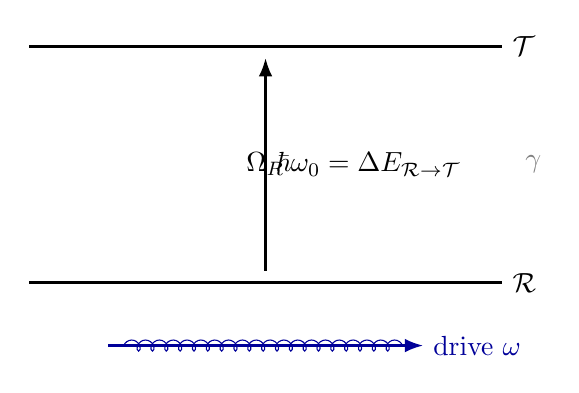
\begin{tikzpicture}[>=Latex,scale=1.0]
    % Energy levels
\draw[very thick] (0,0) -- (6,0) node[right] {$\mathcal R$};
\draw[very thick] (0,3) -- (6,3) node[right] {$\mathcal T$};
% Transition arrow
\draw[->,thick] (3,0.15) -- node[right] {$\hbar\omega_0=\Delta E_{\mathcal R\to\mathcal T}$} (3,2.85);
% Driving field
\draw[->,thick,blue!60!black] (1,-0.8) -- (5,-0.8) node[right] {drive $\omega$};
\draw[blue!60!black,decorate,decoration={coil,aspect=0.8,segment length=5pt,amplitude=2pt}] (1.2,-0.8) -- (4.8,-0.8);
% Rabi label
\node at (3,1.5) {$\Omega_R$};
% Damping
\node[gray] at (6.4,1.5) {$\gamma$};
\end{tikzpicture}
\caption{Two-level SST manifold for $\mathcal R \leftrightarrow \mathcal T$ with Rabi drive.
At resonance $\omega=\omega_0$, the knotting probability oscillates at $\Omega_R$ and decays at rate $\gamma$, enabling pump--probe control of collapse within an interferometer.}
\label{fig:RabiRT}
\end{figure}
    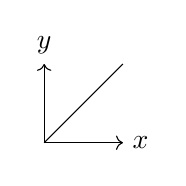
\begin{tikzpicture}
        \draw[->] (0,0) -- (1,0) node[right] {$x$};
        \draw[->] (0,0) -- (0,1) node[above] {$y$};
        \draw (0,0) -- (1,1);
    \end{tikzpicture}


    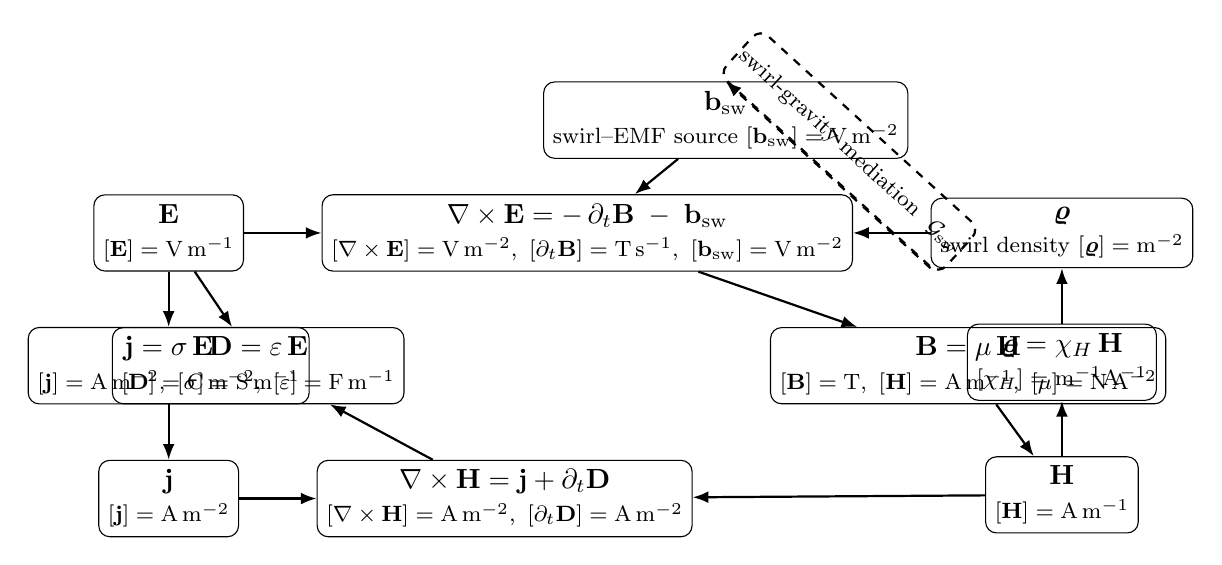
\begin{tikzpicture}[
        node distance=2em and 2.8em,
        every node/.style={draw, rounded corners, align=center, minimum height=2.2em},
        arrow/.style={-{Latex[length=2mm]}, thick},
        garrow/.style={-{Latex[length=2mm]}, thick, dashed} % gravity-mediation link
    ]
    % ===================== NODES =====================
    \node(Faraday)
    {$\nabla \times \mathbf{E} = -\,\partial_t \mathbf{B} \;-\; \mathbf{b}_{\mathrm{sw}}$\\
    \footnotesize $[\nabla\times\mathbf E]=\mathrm{V\,m^{-2}},\ [\partial_t\mathbf B]=\mathrm{T\,s^{-1}},\ [\mathbf b_{\mathrm{sw}}]=\mathrm{V\,m^{-2}}$};

    \node[left=of Faraday]  (E)
    {$\mathbf{E}$\\ \footnotesize $[\mathbf E]=\mathrm{V\,m^{-1}}$};
    \node[right=of Faraday] (rho)
    {$\bm{\varrho}$\\ \footnotesize swirl density $[\bm{\varrho}]=\mathrm{m^{-2}}$};

    \node[below=of rho] (C)
    {$\bm{\varrho} = \chi_H\,\mathbf{H}$\\
    \footnotesize $[\chi_H]=\mathrm{m^{-1}A^{-1}}$};

    \node[below=of E] (Ohm)
    {$\mathbf{j} = \sigma\,\mathbf{E}$\\
    \footnotesize $[\mathbf j]=\mathrm{A\,m^{-2}},\ [\sigma]=\mathrm{S\,m^{-1}}$};

    \node[below right=2em and -3em of Faraday] (B)
    {$\mathbf{B}=\mu\,\mathbf{H}$\\
    \footnotesize $[\mathbf B]=\mathrm{T},\ [\mathbf H]=\mathrm{A\,m^{-1}},\ [\mu]=\mathrm{N\,A^{-2}}$};
    \node[below left=2em and -3em of Faraday] (D)
    {$\mathbf{D}=\varepsilon\,\mathbf{E}$\\
    \footnotesize $[\mathbf D]=\mathrm{C\,m^{-2}},\ [\varepsilon]=\mathrm{F\,m^{-1}}$};

    \node[below=of Ohm] (J)
    {$\mathbf{j}$\\ \footnotesize $[\mathbf j]=\mathrm{A\,m^{-2}}$};

    \node[right=of J] (Ampere)
    {$\nabla \times \mathbf{H} = \mathbf{j} + \partial_t \mathbf{D}$\\
    \footnotesize $[\nabla\times\mathbf H]=\mathrm{A\,m^{-2}},\ [\partial_t\mathbf D]=\mathrm{A\,m^{-2}}$};

    \node[below=of C] (H)
    {$\mathbf{H}$\\ \footnotesize $[\mathbf H]=\mathrm{A\,m^{-1}}$};

    \node[above left=1.4em and 0.8em of rho] (b)
    {$\mathbf{b}_{\mathrm{sw}}$\\ \footnotesize swirl–EMF source $[\mathbf b_{\mathrm{sw}}]=\mathrm{V\,m^{-2}}$};

    % ===================== ARROWS =====================
    \draw[arrow] (E) -- (D);
    \draw[arrow] (C) -- (rho);
    \draw[arrow] (rho) -- (Faraday);
    \draw[arrow] (J) -- (Ampere);
    \draw[arrow] (H) -- (Ampere);
    \draw[arrow] (E) -- (Faraday);
    \draw[arrow] (Faraday) -- (B);
    \draw[arrow] (Ampere) -- (D);
    \draw[arrow] (B) -- (H);
    \draw[arrow] (H) -- (C);
    \draw[arrow] (E) -- (Ohm);
    \draw[arrow] (Ohm) -- (J);

    % ===== SWIRL-GRAVITY (dashed) =====
    \draw[garrow] (rho.south west) -- node[above,sloped,inner sep=1pt]
        {\footnotesize swirl-gravity mediation $\ \mathcal{G}_{\mathrm{sw}}$}
    (b.north);

    \draw[arrow] (b) -- (Faraday);
    \end{tikzpicture}


\end{document}